\documentclass[journal,12pt,twocolumn]{IEEEtran}
\usepackage{amsmath,amsfonts,amssymb,float,gvv,graphicx,enumitem,array,esint}
\bibliographystyle{IEEEtran}
\vspace{3cm}
\title{NCERT Discrete}
\author{Pragnidhved Reddy\\EE23BTECH11050}
\date{}
\parindent 0px
\begin{document}
\maketitle
\newpage
\bigskip
\textbf{Question 11.9.3.18:}\\
 Find the sum to n terms of the sequence $8,88,888,8888$\ldots\\
 \solution \\
 \begin{table}[H]
\centering
\setlength{\extrarowheight}{8pt}
\begin{tabular}{|c|c|c|}\hline
\textbf{Parameter} & \textbf{Value} & \textbf{description}\\ \hline
$x\brak{0}$ & 8 & First term \\ \hline
$x\brak{1}$ & 88 & Second term \\ \hline 
$x\brak{n}$ & $(\sum^{n}_{k=0}8\brak{10^k}u\brak{n}$ & General term \\ \hline
$S\brak{n}$ & $S\brak{n}=\sum^{n-1}_{k=0}x\brak{k}$ & Sum of n terms \\ \hline
\end{tabular}
\caption{Input parameters}
\label{tab:table1}
\end{table}
 From \eqref{tab:table1}
\begin{align}
\label{eq:eq5}
 s\brak{n}&=x\brak{n}* u\brak{n}
 \end{align}
 Z transform of general term
 \begin{align}
 X\brak{z}&=\sum_{n=-\infty}^{\infty}(\sum_{k=0}^{n}8(10)^k)u\brak{n}z^{-n}\\[6pt]
 X\brak{z}&=8\sum_{n=0}^{\infty}\left(\sum_{k=0}^{n}(10)^k\right)u\brak{n}z^{-n}\\[6pt]
 X\brak{z}&=8\left(\sum_{n=0}^{\infty}(10)^n(z^{-n})\right)\left(\sum_{n=0}^{\infty}z^{-n}\right)\\
 \implies X(z)&=\left(\frac{8}{(1-10z^{-1})(1-z^{-1})}\right) \quad \abs{z}>10
\end{align}
From \eqref{eq:eq5}, we get
 \begin{align}
 S\brak{z}&=(X\brak{z})(U\brak{z})\\
 S\brak{z}&=\left(\frac{8}{(1-10z^{-1})(1-z^{-1})}\right)\left(\frac{1}{1-z^{-1}}\right)\\[6pt]
 S\brak{z}&=\left(\frac{8}{(1-10z^{-1})(1-z^{-1})^2}\right)
\end{align}
\begin{align}
 S\brak{z}&=\frac{-224z^{-1}}{81(1-z^{-1})}-\frac{8z^{-2}}{9(1-z^{-1})^2}+\frac{8000z^{-1}}{81(1-10z^{-1})}+8
 \end{align}
 \begin{align}
\label{eq:eq11}
\delta (n) &\overset{Z}\longleftrightarrow 1\\
\label{eq:eq12}
u \brak {n-1}&\overset{Z}\longleftrightarrow\frac{z^{-1}}{1-z^{-1}} \quad \abs{z} > 1 \\
\label{eq:eq13}
a^{n-k}u\brak{n-k}&\overset{Z}\longleftrightarrow\frac{z^{-k}}{1-az^{-1}} \quad \abs{z} > a \\
\label{eq:eq14}
\brak{n-k}u\brak{n-k}&\overset{Z}\longleftrightarrow\frac{z^{-k-1}}{\brak{1-z^{-1}}^2} \quad \abs{z} > 1 
\end{align}
From the above 4 equations, we get
 \begin{align}
 \notag s\brak{n}&=\frac{-224u\brak{n-1}}{81}-\frac{8\brak{n-1}u\brak{n-1}}{9}\\&~~~~~~~
 +\frac{8000(10^{n-1})u\brak{n-1}}{81}+8\delta \brak{n}
\end{align}
\begin{figure}[h!]
    \centering
    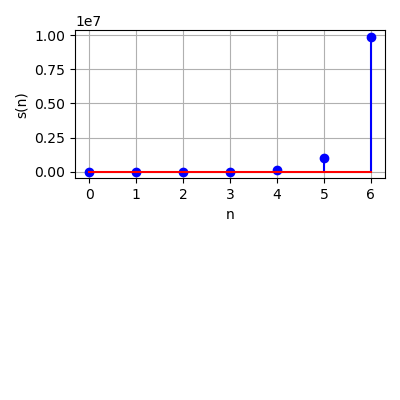
\includegraphics[width=\columnwidth]{figs/plot.png}
    \caption{graph of sum of n terms}
    \label{fig:1}
\end{figure}
 \end{document}
